\documentclass{llncs}
\usepackage{graphicx,psfig,amsmath,float,epstopdf,multirow,mathtools,changepage,amssymb}
\usepackage[para,online,flushleft]{threeparttable}
\usepackage{float} % lets you have non-floating floats
\usepackage{url} % for typesetting urls
\usepackage{caption}
\usepackage{program}
\usepackage{tabularx}
\usepackage{colortbl}
\usepackage{algorithm, algpseudocode}

%\usepackage{mathtools}
\usepackage{etoolbox}
\usepackage{hhline}
\usepackage{subcaption}
\newfloat{fig}{thp}{lof}[section]
\floatname{fig}{Figure}
\let\bbordermatrix\bordermatrix
\patchcmd{\bbordermatrix}{8.75}{4.75}{}{}
\patchcmd{\bbordermatrix}{\left(}{\left[}{}{}
\patchcmd{\bbordermatrix}{\right)}{\right]}{}{}


\title{
Optimization of Location Allocation of Web Services Using A Modified Non-dominated Sorting Genetic Algorithm
}

\author{Boxiong Tan, Hui Ma, Mengjie Zhang}
\institute{School of Engineering and Computer Science,
\\Victoria University of Wellington, New Zealand \\
\email{\{Boxiong.Tan, Hui.Ma, Mengjie.Zhang\}@ecs.vuw.ac.nz}}

\makeatletter
\usepackage[pdfauthor={\@author}, pdftitle={\@title}]{hyperref}
\makeatother

\begin{document}

\maketitle

\begin{abstract}
In recent years, web services technology is becoming increasingly popular because of the convenience, 
low cost and capacity to be composed into high-level business processes. 
The service location-allocation problem for a web service provider is critical and urgent,
because some factors such as network latency can make serious effect on the quality of service (QoS). 
This paper presents a multi-objective optimization algorithm based on NSGA-II to solve the service location-allocation problem. 
A stimulated experiment is conducted using the WS-DREAM dataset. 
The results are compared with a single objective genetic algorithm (GA). 
It shows NSGA-II based algorithm can provide a set of best solutions that outperforms genetic algorithm.
\end{abstract}

\section{Introduction}
Web Services are considered as self-contained, self-describing, modular applications that can be published, located, and invoked across the Web \cite{Ran}. 
In recent years, web services technology is becoming increasingly popular because of the convenience, low cost and capacity to be composed into high-level business processes \cite{Aboolian}.

With the ever increasing number of functional similar web services being available on the Internet, the web service providers (WSPs) are trying to improve the quality of service (QoS) to become competitive in the market.  
QoS, also known as non-functional requirements to  web services, is the degree to which a service meets specified requirements or user needs \cite{4061431}, such as response time, security and availability. 
Among numerous QoS measurements, service response time is a critical factor for many real-time services, e.g. traffic service or finance service. 
Service response time has two components: transmission time (variable with message size) and network latency \cite{Johansson}. 
Study \cite{916684} shows that network latency is a significant component of service response delay.
Ignoring network latency will underestimate response time by more than 80 percent \cite{Sun}, since network latency is related to network topology as well as physical distance \cite{distanceMetrics}. 
To reduce the network latency WSPs need to allocate services location where has the lower latency to the user center that
access the services. Ideally, WSPs could deploy their services to each user center in order to provide the best quality.
However, the more services deployed, the better the quality and the higher cost. 


The Web service location-allocation problem is essentially a multi-objective optimization problem \cite{Multiobjective}, for which there are two conflict objectives, to provide optimal 
QoS to service users and to consume minimal deployment cost.
This problem is considered as NP-hard due to the fact that the combinatorial explosion of the search space \cite{Vanrompay}. 


Very few researches have studied the service location-allocation problem and most of the researchers treat this problem as a single objective problem.
\cite{Aboolian} \cite{Sun} try to solve the problem by using integer linear programming techniques.
In particular, \cite{Sun} solved this problem by employing greedy and linear relaxations of Integer 
transpotation problem.
However, the major problem for this approach is that linear programming is not scaling.
%As a result, the solution is easily stuck at local optima.
Huang \cite{EnhancedGenetic} proposed an enhanced genetic algorithm (GA)-based approach, which make use of the integer scalarization technique to solve this problem.
%GA \cite{man1996genetic} is an Evolutionary algorithm (EA) that uses genetic operators to obtain optimal solutions without any assumptions about the search space.
This algorithm solves the problem with one objective and one constraint. However there has some deficiencies in the
integer scalarization techniques \cite{Multiobjective}. Firstly, the decision maker needs to choose an appropriate weights for the objectives to retrieve a satisfactorily solution. 
Secondly, non-convex parts of the Pareto set cannot be reached by minimizing convex combinations of the object functions.


So far, to the best of our knowledge, there is no research has considered the service location-allocation problem as a multi-objective problem. Therefore, this paper we will treat service location-allocation problem as a multi-objective problem. Evolutionary multi-objective optimization (EMO) methodologies
 is ideal for solving multi-objective optimization problems \cite{key:article}, since EMO works with a population of solutions and 
a simple EMO can be extended to maintain a diverse set of solutions.
With an emphasis for moving toward the true Pareto-optimal region, an EMO can be used to find multiple Pareto-optimal solutions in 
one single simulation run \cite{OptimizationElectrical}. Among numerous EMO algorithms,
Non-dominated sorting GA (NSGA-II) \cite{996017}, Strength Pareto Evolutionary Algorithm 2 (SPEA-2) \cite{Deb} have become standard approaches. 
Some schemes based on particle swarm optimization (PSO) approaches are also proposed \cite{Elhossini} \cite{Huang}.
NSGA-II is one of the most widely used methods for generating the Pareto frontier, because it can keep diversity without specifying any additional parameters \cite{Deb06referencepoint}.
In this paper, we propose to use NSGA-II to solve the web service location-allocation problem, which has two objectives:
cost and network latency.


%
%To show the effective and efficiency of our proposed NSGA-II based approach, we conduct an experiment to compare our approach with
%traditional approach based on integer programming and greedy optimization (IPGO). IPGO models one objective as an assignment problem then uses integer programming techniques to 
%obtain an optimal solution. Then, based on this solution, the algorithm further optimize the other objective using greedy algorithm. 
%The major advantage of IPGO is that it is very efficient and gives 
%an reasonably good result. On the other hand, the objectives are considered unevenly. That is, IPGO considers the objective which optimize by linear programming as its priority.
%

%The aim of this research is to provide a framework that guides a WSP to locate services.
We consider the problem faced by a WSP who has existing facilities but wishes to use the collected data to re-allocate their services in order to maximum their profit.
The WSP must decide on facility locations from a finite set of possible locations. 
In order to make a decision, the WSP must first analyze the data collected from current use of services. 
The collected data should includes the records of invocations from each unique IP address.
Therefore, based on these data, the WSP could summarize several customer demands concentrated on \textit{n} discrete nodes \cite{Aboolian}, namely user centers. 
We assume that the WSP has already done this step and a list of user centers and candidate service deployment locations are given.
In addition to deciding locations to of the services, information about network latency between user centers and candidate locations is needed. 
Exist datasets in \cite{6076756} \cite{5552800} contain latency information collected from the real world. 

The aim of this project is to propose a NSGA-II based approach to produce a set of near optimal solutions of service location-allocation, so that cost and overall network latency are 
close to minimum. Then, the service provider could use the algorithm which proposed by this paper, to select an optimal plan based on their funds. 
The main objectives are:
\begin{itemize}
	\item To model the web service location-allocation problem so that it can be tackled by NSGA-II.
	\item To develop a NSGA-II based approach to the web service location-allocation problem.
	\item To evaluate our proposed approach using some existing datasets.
	%\item To evaluate our approach by comparing it to a linear assignment with greedy optimization (IPGO) algorithm.
\end{itemize}

In Section \ref{sec:Background} we introduce the background of NSGA-II and GA.
In Section \ref{sec:problem} we provide models of the service location allocation problems. Section \ref{sec:algorithm_des} develops a NSGA-II based algorithm. 
%We use these to study a number of hypotheses on the placement of WSPs. These solutions are compared to solutions from Integer
%programming with greedy optimization(IPGO). 
The experimental design and results evaluation are shown in Section \ref{sec:experiment}. Section \ref{sec:conclusion} provides a brief summary.


\section{Background}
\label{sec:Background}
%A few researchers attempt to solve the service location-allocation problem by using a single objective approach. Most of them solve this problem with linear programming approaches.
%\cite{5961695} considers more than 3 objectives: response time, availability and cost. 
%It solves the placement of data centers for Internet Services with simulated annealing plus linear programming. 
%Sun et.al proposed two approaches \cite{Aboolian} \cite{Sun} that employ LP and DAL respectively. 
%The first approach \cite{Aboolian} assumes the model is based on a duopoly competitive market.
%The second approach \cite{Sun} assumes multiple competition services have been established in the market.
%Some researchers use evolutionary algorithms. Huang \cite{EnhancedGenetic} applied an enhanced GA algorithm which employ the integer scalarization technique \cite{Multiobjective}. However, 
GA \cite{man1996genetic} is a powerful tool to solve combinatorial optimization problems. It is an iterative procedure based on a constant-size population. In a GA, a population of strings (called chromosomes
or the genotype of the genome), which are encoded as candidate solutions (called individuals, creatures, or phenotypes) to an optimization problem, evolves towards better solutions. 
Each genome is associated with a fitness value based on a fitness function that indicates how close it comes to meeting the overall specification, when compared to other genomes in the
population. The fitness value of an individual is also an indication of its chances of survival and reproduction in the next generation. A typical genetic algorithm requires a genetic
representation of the solution domain and a fitness function to evaluate the solution domain. Since a chromosome from the population represents a solution, when the algorithm starts, 
the whole population moves like one group towards an optimal area so the GA searches from a population of solutions rather than a single solution. Integer scalarization technique \cite{Multiobjective} is 
used to solve multi-objective problems with GA. It predefines a weight for each objective.

NSGA-II is a multi-objective algorithm based on GA. When used for problems with only two objectives, NSGA-II performs 
relatively well in both convergence and  computing speed. It permits a remarkable level of flexibility with regard to 
performance assessment and design specification. NSGA-II assumes that every chromosome in the population has two 
attributes: a non-domination rank in the population and a local crowding distance in the population. The goal of 
NSGA-II is to converge to the Pareto front as possible and with even spread of the solutions on the front by 
controlling the two attributes. 

The algorithm starts with a random initialization population. Once the population is sorted based on non-domination sorting, a rank is assigned to each chromosome.
Then, a parameter called crowding distance is calculated for each individual. The crowding distance is a measure of how close an individual is to its neighbors. A large 
average crowding distance will result in better diversity in the population. 

Parents are selected from the population by using tournament selection based on the rank and the crowding distance. An individual is selected in the rank if it is smaller than the other or 
if the crowding distance is greater than the other. The selected population generates offsprings using crossover and mutation operators. 

The population with the current population and current offsprings is sorted again based on non-domination and only the best N individuals are selected, where N is the population size.
The selection is based on rank and the on crowding distance on the last front.

%\subsection{Integer programming with Greedy Optimaization (IPGO)}
%
%Linear assignment \cite{lawler1963quadratic} is a special case of the transpotation problem, which is a special case of the minimum cost flow problem, which
%in turn is a special case of a linear program.
%
%Much research has been devoted to develop efficient heuristic algorithm to solve location-allocation problem. Two of the predominant
%greedy construction heuristics are the ADD and DROP \cite{Sun} methods, which build solutions from scratch. 
%The ADD procedure starts with all facilities closed and locates a facility that gives the greatest savings at each step and 
%iterates through all potential locations until no further savings can be made. In contrast, DROP opens all facilities and removes a 
%location that gives the greatest savings at each step and tries to find optimal or near optimum solutions at the end of the 
%iterative procedure. Integer programming with greedy optimization(IPGO) builds upon ADD and DROP methods. 
%In order to solve multi-objective problem, IPGO first employs Integer programming to derive a minimum cost solution, it then 
%uses a greedy procedure to optimize the other objective.
%
%Sun et al. proposed Drop, ALA, and LP relaxations of Integer transpotation problem (DAL) \cite{Sun} is very similar with this approach. 
%The DAL heuristics provided near optimal solutions in short computer times and with limited computer memory. But in Sun's approach, 
%he assumes there is competitive service providers existed. In contrast, IPGO does not consider about existed services. Therefore, IPGO
%uses Linear assignment approach instead of Alternate Location-allocation (ALA).
%
%
%
\section{Problem Description and Modeling}
\label{sec:problem}
In this section, we first describe the service location-allocation problem, then we will present models for the services location allocation problem.

\subsection{Problem Description}
Web service location-allocation problem is to determine reasonable locations for web services so that the deployment cost of WSP can be minimized while service performance can be optimized.
In this paper, to optimize service performance we consider to minimize network latency.

The task of service location allocation has two objectives:
\begin{itemize}
	\item To minimize the total cost of the services.
	\item To minimize the total network latency of the services.
\end{itemize}


\subsection{Model Formulation}
\label{sec:model}
To model service location-allocation problem, we need to make use of a set of matrices, to present input information and output solutions. 

For service location-allocation problem, we need information of service usage, network latency, and service deployment cost to decide service location-allocation so that the overall network latency can be minimized with minimal deployment cost and within constraints.
Assume a set of $S = \{ s_{1}, s_{2}, ...s_{s}, s_{x}\}$ services are
requested from a set of locations $I = \{ i_{1}, i_{2}, ...i_{i}, i_{y} \}$. 
The service providers allocate services to the set of candidate facility locations $J = \{ j_{1}, j_{2}, ...j_{j}, j_{z} \}$.


In this paper, we will use the following matrices.
\begin{center}
{
%\centering
	\begin{tabular}{l*{2}{l}r}
		\hline
		\textbf{Matrices} \cr
		$L$ & server network latency matrix $L = \{l_{ij}\}$ \cr
		$A$ & service location matrix $A = \{a_{sj}\}$ \cr
		$F$ & service invocation frequency matrix $F = \{f_{is}\}$ \cr
		$C$ & cost matrix $C = \{c_{sj}\}$ \cr
		$R$ & user response time matrix $R = \{r_{is}\}$ \cr
		\hline
	\end{tabular}
%\\
}
\end{center}
A \emph{service invocation frequency matrix}, $F= [f_{is}]$, is used to record services invocation frequencies from user centers, 
where $f_{is}$ is an integer that indicates the number of invocations in a period of time from a user center to a service. 
For example, $f_{13}$ = 85 denotes service $s_{1}$ is called 85 times in a predefined period of time.

\parbox{.45\linewidth}{
{\centering
$
F = \bbordermatrix{~ & s_{1} & s_{2} & s_{3}  \cr
					i_{1}	&120 &35 &56	\cr
					i_{2}	&14  &67 &24 \cr
					i_{3}	&85 &25 &74 \cr}
$
\\}
}
\parbox{.45\linewidth}{
{\centering
$
L = \bbordermatrix{~ & j_{1} & j_{2} & j_{3} \cr
					i_{1}	&0 &5.776 &6.984	\cr
					i_{2}	&5.776  &0 &2.035 \cr
					i_{3}	&0.984 &1.135	&2.3 \cr}
$
\\}
}

A \emph{network latency matrix} $L = [l_{ij}]$, is used to record network latencies from user centers to 
candidate locations. For example, The network latency between user center $i_{2}$ with candidate location $j_{1}$ 
is 5.776s. These data could be collected by monitoring network latencies \cite{6076756} \cite{5552800}.

The cost matrix $C = [c_{sj}]$, is used to record the cost of deployment of services to candidate locations, 
where $c_{sj}$ is an integer that indicate the cost of the deploying a service to a location. 
For example, $c_{12} = $ 80 denotes the cost of deploying service $s_{1}$ to location $j_{2}$ is 80 cost units.

\parbox{.45\linewidth}{
{\centering
$
C = \bbordermatrix{~ & j_{1} & j_{2} & j_{3}\cr
					s_{1}	&130 &80 &60\cr
					s_{2}	&96  &52 &86\cr
					s_{3}	&37 &25 &54\cr}
$
\\}
}
\parbox{.45\linewidth}{
{\centering
$
A = \bbordermatrix{~ & j_{1} & j_{2} & j_{3}\cr
					s_{1}	&0 &1 &0	\cr
					s_{2}	&0  &0 &1	\cr
					s_{3}	&1 &1 &0	\cr}
$
\\}
}

To model the service location-allocation problem, we consider the following assumptions:
\begin{enumerate}
	\item The new WSP decides where to locate his facilities regardless of there is existed functional similar services from other WSPs.
	\item The decision of service location-allocation is made only considering two factors: total network latency and total cost.
	\item A static allocation policy is used by WSPs. In practice, Web services typically offer clients persistent and interactive services, which often span over multiple sessions. Therefore, a dynamic reallocation scheme is not practical as it may disrupt the continuity of the services.
\end{enumerate}


A \emph{service location-allocation matrix} $A = [a_{sj}]$ represents the actual service location-allocation, where $a_{sj}$  is a binary value 1 or 0 to indicate whether a service is allocate to a location or not.


Using service location allocation matrix $A = [a_{sj}]$ and network latency matrix $L = [l_{ij}]$, we can compute user
response time matrix $R = [r_{is}]$, 

{\centering
	\begin{equation}
		r_{is} = MIN\{l_{ij} \mid j \in \{1, 2, ..., z\} \text{ and } a_{sj} = 1\}
	\end{equation}
\\}
For example, we can use the two example matrices $L$ and $A$ presented above to construct the response time matrix $R$. 
For each service $s$, by checking matrix $A$, we can find out which location the service has been deployed.
Then look back matrix $L$, find out its corresponding latency to each user center $i$. If there is
more than one location, then the smallest latency is selected. Therefore, we can construct the response time matrix $R$ as:

{\centering
$
R = \bbordermatrix{~ & s_{1} & s_{2} & s_{3}\cr
					i_{1}	&5.776 &6.984 &0	\cr
					i_{2}	&0  &2.035 &0	\cr
					i_{3}	&1.135 &2.3 &0.984	\cr}
$
\\}


\section{NSGA-II for Web Services Location Allocation}
\label{sec:algorithm_des}
To apply NSGA-II to the service location-allocation problem, the first step is to define the variable in NSGA-II, i.e. to
identify chromosome, genetic operators and the fitness functions.

\subsection{Chromosome Representation and Constraints}
In our approach, we model the service location matrix $A$ = $[a_{sj}]$ as a chromosome that we mentioned in Section 
\ref{sec:problem}.

The constraint setting is based on service providers' needs. One can set multiply constraints to the problem to narrow the potential searching space.
In our case, we set two basic constraints. The first constraint service number constraint requires that each service is deployed in at 
least one location.

{\vspace*{0mm}
	\centering
	\begin{equation}
		\sum\limits_{x \in S} a_{xj} \geq 1
	\end{equation}
\\}

The second constraint, is cost constraint, which sets up  the upper boundary of the total cost.
An integer number $CostLimitation$ is decided by the WSP.

{\vspace*{0mm}
	\centering
	\begin{equation}
		\sum\limits_{s \in S} \sum\limits_{j \in J} c_{sj} \times a_{sj} \leq CostLimitation
	\end{equation}
\\}


\subsection{Genetic Operators}
\label{sec:operators}
 The original NSGA-II uses a simulated 
binary crossover (SBX) \cite{930314} and polynomial mutation \cite{Raghuwanshi04} 
to cope with continuous problems. 
However, our problem is discretized, therefore we use the regular GA mutation and crossover operations.

The selection operator is the tournament selection \cite{Xie:2008:AMI:1389095.1389347}, which allows the highest probability 
of being reproduced to next generation.

\begin{flushleft}\textbf{Mutation} The mutation operator works as follows: initially choose one random location from the chromosome. 
Then, this location is replaced by by its inverse value e.g 1 to 0 or 0 to 1.
\end{flushleft}

In this study, a chromosome in a population will be selected based on mutation possibility $P_{m}$, which is 
a parameter predefined and fixed.
%As shown in below, a random position will be selected and replaced by a reversed number.
\begin{figure}[ht]
\centering
	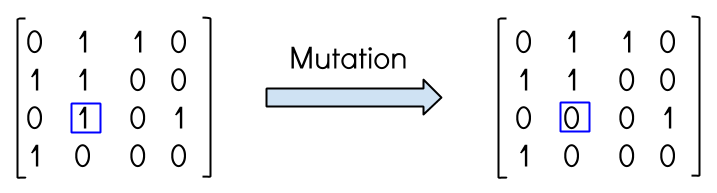
\includegraphics[width=0.5\textwidth]{pics/mutation.png}
\caption{}
\label{graph1}
\end{figure}
\begin{flushleft}\textbf{Crossover} The crossover operator in this paper is the single point crossover. 
The crossover is controlled by crossover probability $P_{c}$, is a parameter predefined and fixed.
The crossover point is created randomly within the length of the chromosome. 
\end{flushleft}
%As in the example below, two parents crossover at a point, to generate two offsprings.
\begin{figure}[ht]
\centering
	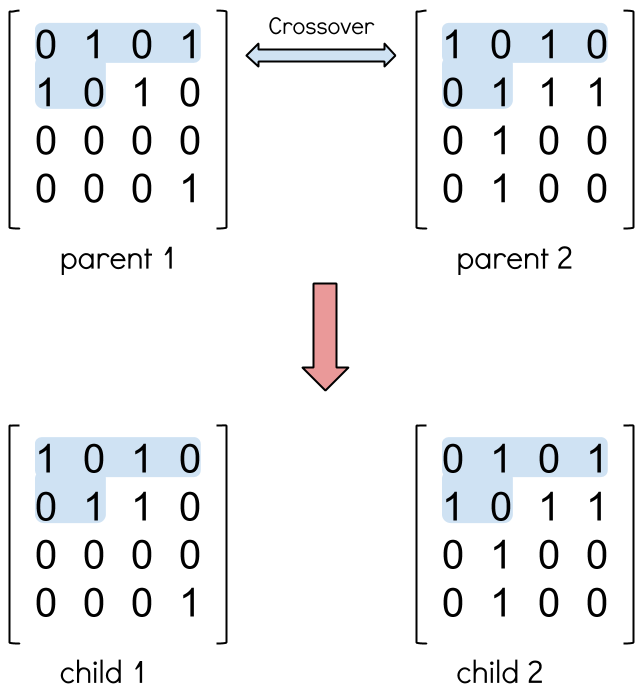
\includegraphics[width=0.5\textwidth]{pics/crossover.png}
\caption{}
\label{graph2}
\end{figure}

\subsubsection{Fitness Function}
\label{sec:fitness_functions}
\begin{flushleft}In order to accomplish these two objectives, we design two fitness functions to evaluate 
how good each chromosome meets the objectives. We use CostFitness to calculate the overall cost of deploying services under an allocation plan\end{flushleft}
%\subsubsection{Cost fitness function}

\begin{equation}
	CostFitness = \sum\limits_{s \in S} \sum\limits_{j \in J} c_{sj} \times a_{sj}
\end{equation}

\begin{flushleft}$c_{sj}$ is the cost of deploying service $s$ at location $j$, where $a_{sj}$ represents the deployment plan. The sum of the multiplication of 
$c_{sj}$ and $a_{sj}$ is the total deployment cost.\end{flushleft}


%\begin{flushleft}For example, we use the above mentioned matrices $C$ and $A$.\end{flushleft}

	%$
	%CostFitness &= c_{11} * a_{11} + c_{12} * a_{12} + c_{13} * a_{13} + ... + c_{33} * a_{33} \\
	%&= 130 * 0 + 80 * 1 + 60 * 0 + ... + 54 * 0 \\
	%&= 228
	%$
We assume the latency is symmetrical between user center and candidate location. e.g. 
The latency from location $i$ to location $j$ is same with the latency from location $j$ to location $i$.

	\begin{equation}
		LatencyFitness = \sum\limits_{i \in I} \sum\limits_{s \in S} r_{is} \times f_{is}
	\end{equation}

\subsubsection{Normalise function}
To indicate the goodness of an allocation solution we normalise CostFitness and LatencyFitness according to the largest and minimum values of
CostFitness and LatencyFitness. Normalised fitness values can also be used to compare results from different approaches.
Since the maximum and minimum value for total cost and total latency are deterministic, we use exhaustive search to
find out the $Latency_{max}$. $Latency_{min}$ is zero for we assume each service could be deployed in each user center. 
$Cost_{min}$ is the cost of allocation each of services at a location that leads to minimal cost and $Cost_{max}$ is the cost of allocation when each service is allocated to all the 
locations.
	\begin{equation}
		CostFitness^\prime = \frac{CostFitness - Cost_{min}}{Cost_{max} - Cost_{min}}
	\end{equation}

	\begin{equation}
		LatencyFitness^\prime = \frac{LatencyFitness - Latency_{min}}{Latency_{max} - Latency_{min}}
	\end{equation}
%\begin{flushleft}For example, we use the above mentioned matrices F and R.\end{flushleft}

	%$
	%LatencyFitness &= f_{11} * r_{11} + f_{12} * r_{12} + f_{13} * r_{13} + ... + f_{33} * r_{33} \\
	%&= 120 * 5.776 + 6.984 * 35 + 0 * 56 + ... + 0.984 * 74\\
	%&= 1300.696
	%$



\subsection{NSGA-II based algorithm for service location-allocation}
%Algorithm \ref{NSGA2} shows the precedure of NSGA-II applied on service location-allocation problem.
\begin{algorithm}[htb]
	\caption{NSGA-II for service location-allocation}
	\label{NSGA2}
	\textbf{Inputs:}
		Cost Matrix $C$,
		Server network latency matrix $L$, 
		Service location matrix $A$, 
		Service invocation frequency matrix $F$

	\textbf{Outputs:}
		Pareto Front:a  set of service allocation matrix $A$

	\begin{algorithmic}[1]
		\State Initialize a population of chromosome with random binary values
		\State Evaluate population with fitness functions
		\State Non-dominated sort and assign a ranking to each chromosome
		\State Evaluate the Crowding distance of each chromosome
		\State Initialize the Pareto Front Pool
		\While{predefined generation}
		\State Apply Tournament Selection
		\State Apply Crossover 
		\State Apply Mutation
		\For( each chromosome)
		\While{ violate service number constraint}
		\State random choose a location $j$ and set $a_{sj}$ = 1
		\EndWhile
		\While { violate cost constraint}
		\State random choose a location $j$ and set $a_{sj}$ = 0, as long as $\sum\limits_{s \in S} a_{sj} \geq 1$
		\EndWhile
		\If{ chromosome does not exist in the Pareto front Pool}
		\State Evaluate with the fitness functions
		\EndIf
		\EndFor
		\State Non-dominated sort and assign ranking
		\State Evaluate the Crowding distance
		\State Recombination and Selection
		\State Update the Pareto Front Pool with the current Pareto Front
		\EndWhile
		\State Return the Pareto Front
	\end{algorithmic}
\end{algorithm}

There are two major differences between standard NSGA-II and modified version. Firstly, in order to avoid repeatly evaluate the fitness
of chromosome. After the first generation is initialized, the Pareto front will be 
stored in the memory. In each generation, when evaluate the chromosome, the chromosome is checked to see it exists in the memory pool. 
If so, then the calculation of fitness will be skipped. At the end of each iteration, the Pareto front pool is updated to the current Pareto front.
The reason for setting a memory pool is that, after a number of iterations, the population start converging. 
Most of the population are redundant. Therefore, a memory pool could considerably reduce the repeated computation.

The other difference is that, we use general mutation and crossover operation instead of polynomial mutation and simulated binary crossover.
It is important to note that the mutation and crossover operators can produce solutions that might violate the constraints. 
Therefore, repair operators are needed to try to maintain feasible solutions. The proposed algorithm checks the cost and service number constraint to avoid
possible infeasible solutions.

\section{GA for Web Service Location Allocation}
In order to show the advantages of our multi-objective NSGA-II approach, we extend the single-objective algorithm GA based approach in \cite{Huang} to consider two objectives. 
The extended GA-based approach is show as following. A weight $w$ needs to be predefined in GA. The weight is used for 
measuring the importance of objectives. Conventionally, the weight is in the range of $[0, 1]$. In our approach, we define the weight equals 0.5.

\subsubsection{Fitness function}
As in Section \ref{sec:model} we model an allocation matrix as a chromosome. Crossover and mutation operators are same as defined in Section \ref{sec:operators}.
To evaluate the chromosomes of population.
We use Integer Scalarization technique to calculate the fitness value. $w$ is a predefined value to measure the important of cost and latency. Note that CostFitness and LatencyFitness
are calculate in the same as in section \ref{sec:fitness_functions}.

\begin{equation}
		Fitness = w \times CostFitness + (1 - w) \times LatencyFitness
	\end{equation}


\begin{algorithm}[htb]
	\caption{GA for service location-allocation}
	\textbf{Inputs:}
		Cost Matrix $C$,
		Server network latency matrix $L$, 
		Service location matrix $A$, 
		Service invocation frequency matrix $F$, 
		weight parameter $w$

	\textbf{Outputs:}
		One best solution: allocation matrix $A$


	\begin{algorithmic}[1]
		\State Initialize a population of chromosome with random binary value
		\State Evaluate population with the fitness function
		\While{predefined generation}
			\State Apply Tournament Selection
			\State Apply Crossover 
			\State Apply Mutation
			\For( each chromosome)
				\While{ violate service number constraint}
					\State random choose a location $j$ and set $a_{sj}$ = 1
				\EndWhile
				\While { violate cost constraint}
					\State random choose a location $j$ and set $a_{sj}$ = 0, as long as $\sum\limits_{s \in S} a_{sj} \geq 1$
				\EndWhile
			\State Evaluate each chromosome with the fitness function
			\EndFor
			\State Update population
			\EndWhile
		\State Return population
	\end{algorithmic}
\end{algorithm}



%\section{IPGO for Web Service Location Allocation}
%\begin{algorithm}[htb]
	%\textbf{Inputs:}
		%Cost Matrix $C$,
		%Server network latency matrix $L$, 
		%Service location matrix $A$, 
		%Service invocation frequency matrix $F$
%
	%\textbf{Outputs:}
		%Service location matrix $A$
	%\caption{IPGO for service location-allocation}
	%\label{IPGO}
	%\begin{algorithmic}[1]
		%\State initialize allocation matrix $A$ = \{1\}.
		%\State Optimize cost solution $A$ with Integer assignment solver.
		%\State Evaluate Cost fitness with the cost fitness function
		%\For( each row of A)
			%\For( each column of A)
				%\If {$A_{ij}$ = 0}
					%\State Start the service: $A_{ij}$ = 1
					%\State Evaluate $A$ with Network Latency fitness function.
					%\If {Current Network latency fitness is greater than previous fitness}
						%\State Change back $A_{ij}$ = 0
					%\EndIf
				%\EndIf
			%\EndFor
		%\EndFor
		%\State Return Service location matrix $A$
	%\end{algorithmic}
%\end{algorithm}
%In order to solve the location allocation problem with IPGO, we model the cost objective as the priority, optimize with Linear programming.
%The cost matrix $C$ and solution matrix $A$ are identical with the two matrices defined in Section \ref{sec:problem}. We use the same fitness functions as in NSGA-II to 
%evaluate the Cost objective and Latency objective.
%
%\begin{equation}
     %\begin{align}
       %\mbox{Minimize } & \sum\limits_{s \in S} \sum\limits_{j \in J} c_{sj} \times a_{sj} \\
       %\mbox{Subject to} & \\
			%& \sum\limits_{s} A_{sj} = 1 (s = 1, 2, ...),\\
	        %& \sum\limits_{s \in S} \sum\limits_{j \in J} C_{sj} \times A_{sj} \leq CostLimitation \\
		%\mbox{and } & A_{sj} = $0 or 1$ (s, j = 1, 2, ...) \\
     %\end{align}
%\end{equation}

%Once a minimum cost solution is found by linear assignment, the solution set will be passed to the ADD procedure to serve as an initial solution for 
%further improvement on Network latency.
%
 %The ADD procedure as follows:
%\begin{itemize}
	%\item Evaluate network latency fitness of the initial solution.
	%\item Starts a facility then evaluate with network latency fitness function. If the network latency fitness decreased as well as 
		%the cost fitness does not exceed the cost constraint. The solution is kept.
	%\item If there is no location could be choose, terminate the procedure.
%\end{itemize}




\section{Experiment Evaluation}
\label{sec:experiment}
To evaluate the effectiveness and efficiency of our proposed NSGA-II based approach to service location-allocation. We compare our approach with a GA-based single objective approach
using an existing dataset, WS-DREAM \cite{6076756} \cite{5552800}, which is a historical dataset on QoS of Web services from different locations. It contains the data of latency
from 339 different user locations invoked 7824 web services scattered over different locations.

The algorithm was coded in R \cite{Morandat:2012:EDR:2367163.2367172} using existed package: NSGA2R. The program was run on a 3.40GHz 
desktop computer with 8 GB RAM.

4 different service location-allocation problems are designed with different complexities.
\begin{table}[h]
{\centering
	\caption{Complexity table}
	\begin{tabular}{|c|c|c|c|}
		\hline
		\multicolumn{1}{|l|}{problem} & \multicolumn{1}{l|}{user location} & \multicolumn{1}{l|}{server location} & \multicolumn{1}{l|}{number of service} \\\hline
		1                             & 3                                  & 3                                    & 3                                      \\\hline
		2                             & 5                                  & 5                                    & 5                                      \\\hline
		3                             & 10                                 & 10                                   & 10                                     \\\hline
		4                             & 15                                 & 15                                   & 15                                    \\
		\hline
	\end{tabular}
\\}
\end{table}

%To compare with IPGO, four different datasets were used, the problem instance was generated as follows:
	A cost matrix is randomly generated from a normal distribution with mean = 100 and standard deviation = 20, in addition, a frequency matrix was an integer matrix which is randomly generated from a uniform distribution on [1, 120].


In each dataset, algorithms run under four different levels of cost constraints: Sufficient condition is 100\% the expected total cost, 
good condition (70\%), pool condition (40\%) and minimum budget condition (0\%). We try to stimulated a real world budget condition with these four 
scenarios. In the minimum budget condition, 
both algorithms exhaustively reduce the cost until it reaches the service number constraint. The NSGA-II runs 40 independent times with different random 
seeds ranging from 1 to 40. To test the efficiency of the algorithms, We evaluate the average run time for each algorithm. 


Parameter settings for the algorithms are as follow. The population size is 50, and the maximum number of 
generations is 50. The tournament size is 3. 
The crossover probability $P_{c}$ is 0.8 and the mutation probability $P_{m}$ 
is 0.2 as we found that this combination can produce good results. We use same parameter settings for GA. 

To compare with the result of NSGA-II and GA, we first derive the Pareto front by using the approach in \cite{Xue} \cite{6381531}, and then compare the results using approach in \cite{1688438}.
In Xue's approach, NSGA-II generates 40 results (from 40 runs) under each cost constraint 
are presented in the Section \ref{sec:comparison}. 40 sets of solutions 
achieved by each multi-objective algorithm are firstly combined into one union set. GA also generates 40 sets of 
solutions, we select the best one based on its fitness value from each set and combine them into one set. 
The non-dominated solutions are presented to compare with the solutions achieved by GA.

In addition to the comparison between NSGA-II and GA, we conducted full experiments on NSGA-II with an initialisation and GA with an initialisation.
We initialized the population with 49 random chromosomes and a chromosome which leading to minimum cost. We expect the initialized algorithms superior than
the uninitialized algorithms.

\subsection{Effectiveness comparison}
\label{sec:comparison}
We conducted experiments on NSGA-II, GA, NSGA-II with initialisation and GA with initialisation respectively.

We use cost fitness value and latency fitness value as 
x, y coordinate. Our goal is to minimize both cost and latency. Therefore, better solution should locate close to the origin.

Experimental results show that few different cost constraints leads to similar result patterns. Due to the page limitation we shows the results of one cost constraints.
%As a result, these four conditions show similar pattern as in Figure \ref{fig:c1}. 
%The difference between these four scenarios is that the repair operator
%will try to narrow the searching space, hence the solutions will be pushed closer to the y axis.


%not much differences between sufficient condition and minimum condition. On the other hand, 
%The solutions set from GA are clearly inferior than 
%NSGA-II. Especially, when the constraint is restrict, most solutions from GA will be identical. In other words, in minimum condition, the solutions
%from GA lack of diversity.


\begin{figure}[H]
	\centering
	\begin{subfigure}[b]{0.45\textwidth}
		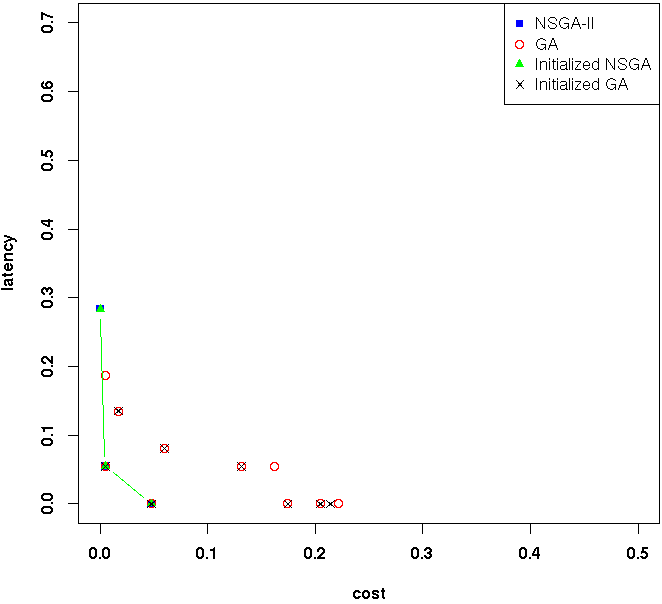
\includegraphics[width=\textwidth]{pics/pop_50_gen_50_3_times_3_sufficient_initialisation.png}
		\caption{3 $\times$ 3}
	\end{subfigure}%
	\begin{subfigure}[b]{0.45\textwidth}
		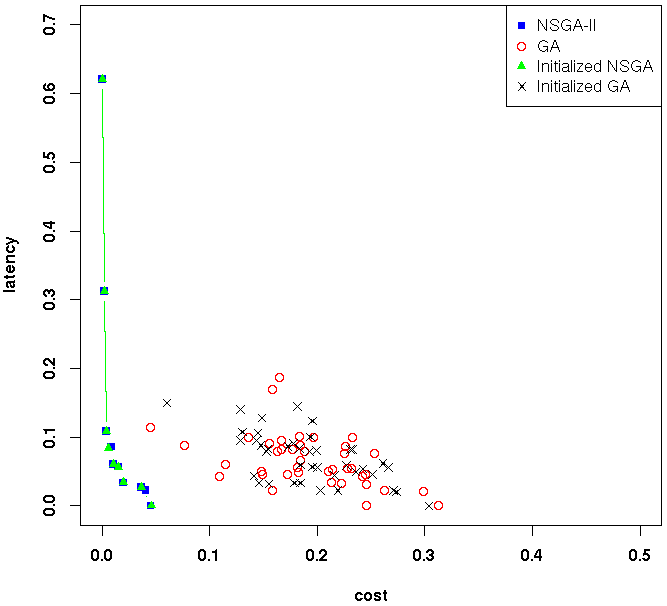
\includegraphics[width=\textwidth]{pics/pop_50_gen_50_5_times_5_sufficient_initialisation.png}
		\caption{5 $\times$ 5}
	\end{subfigure}
	\begin{subfigure}[b]{0.45\textwidth}
		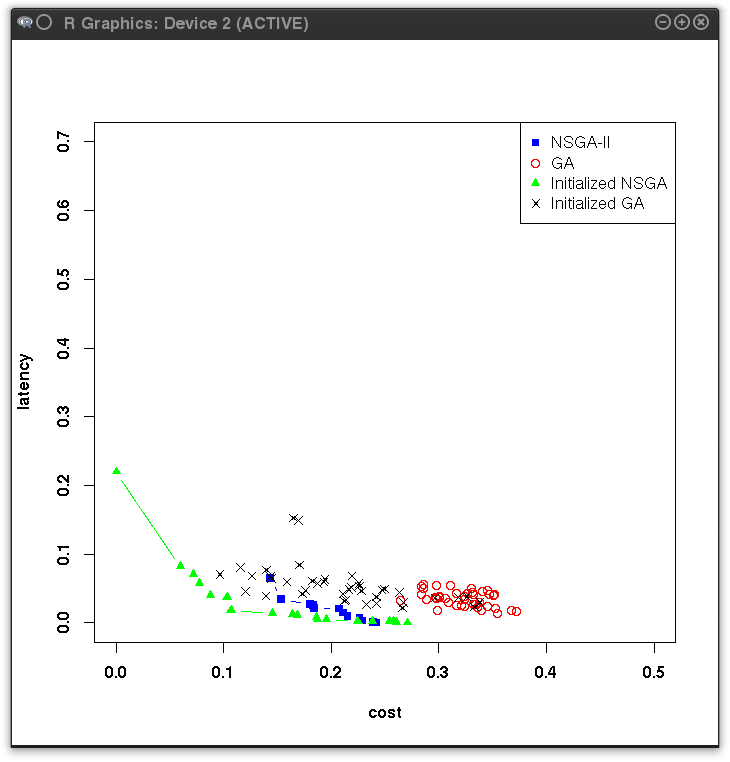
\includegraphics[width=\textwidth]{pics/pop_50_gen_50_10_times_10_sufficient_initialisation.png}
		\caption{10 $\times$ 10}
	\end{subfigure}
	\begin{subfigure}[b]{0.45\textwidth}
		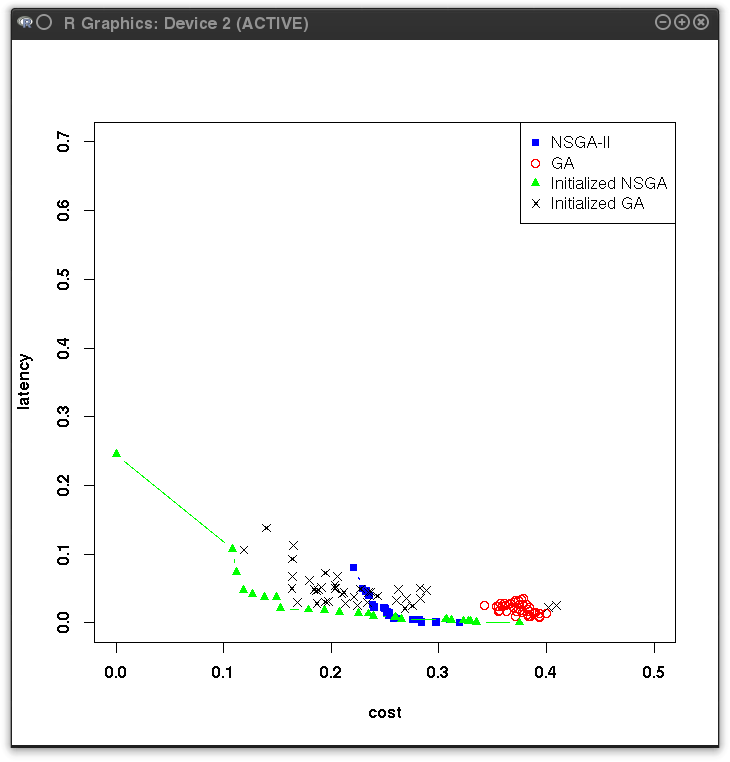
\includegraphics[width=\textwidth]{pics/pop_50_gen_50_15_times_15_sufficient_initialisation.png}
		\caption{15 $\times$ 15}
	\end{subfigure}
	\caption{}\label{fig:c1}
\end{figure}

From the above results we can see that for all the four problems, NSGA-II based approach produces results that dominate or overlap the results from GA based approach. Further,
NSGA-II with an initialized chromosome that represents service location-allocation of the minimum cost dominate the results without a chromosome of the lower cost, though problem 1 and
problem 2 of small complexity size, this observation is not obvious.

In particular, for big problems 3 and 4, results of NSGA-II based approaches dominate the results of GA-based approaches. We also notice that for problems even though the population size
is small as 50, including a chromosome of optimal cost can help to narrow down searching space and to converge to optimal solution faster.
%In 10 $\times$ 10, 15 $\times$ 15 matrices, both results NSGA-II dominate GA, half solutions from initialized GA are better than NSGA-II and initialized NSGA-II still dominate initialized GA.

%The results shows that the algorithms with 50 generation and 50 population are insufficient to an optima solution for such big searching space.
%However, with initialization, both NSGA-II and GA improve their solution significantly. Instead of randomly initializing population, we 
%add one known optima solution into the population could narrow the searching space so that the algorithm could converge faster.




%Figure \ref{fig:3_3} shows NSGA-II outperforms IPGO. As we discussed in the previous section, the 
%result of IPGO is dominated by NSGA-II's solution set. \ref{fig:5_5} \ref{fig:10_10} \ref{fig:15_15} show that solution of IPGO is on the Pareto front. It does not improve the quality of the solution
%set. Therefore, we considered NSGA-II outperforms IPGO in this case. The solution from IPGO is non-dominated solution in the NSGA-II solution set. While the inclusion
%of the IPGO solution somewhat improves the quality of the NSGA-II solution set, we cannot say that IPGO outperforms NSGA-II since the 
%IPGO solution dominates no NSGA-II solutions.

%As a whole, NSGA-II provide a set of solutions not only better than the best solutions from GA but also form a distributed Pareto front.
\subsection{Efficiency comparison}
%\small
\begin{table}[h]
\caption{Efficiency Test}
\scalebox{0.75}{
\begin{tabular}{|l|l|l|l|l|l|l|l|l|l|}
\hline
 & \multicolumn{2}{l|}{$3 \times 3$} & \multicolumn{2}{l|}{$5 \times 5$} & \multicolumn{2}{l|}{$10 \times 10$} & \multicolumn{2}{l|}{$15 \times 15$} \\ \hline
	&	NSGA-II(s)	&	GA(s)	& 	NSGA-II(s)	& 	GA(s)	&  	NSGA-II(s)	&  	GA(s)	& 	NSGA-II(s)	&   GA(s)\\ \hline
Sufficient 		&4.4 $\pm$ 0.3		& 1.6 	$\pm$ 0.1	$\downarrow$& 5.9 $\pm$ 0.1& 3.2 $\pm$ 0.1	$\downarrow$& 13.7 $\pm$ 0.1&11.0 $\pm$ 0.1 & 27.0 $\pm$ 0.1 &23.9 $\pm$0.5$\downarrow$\\ \hline
 Good 			&4.4 $\pm$ 0.2		& 1.6 $\pm$0.1 $\downarrow$     &6.0 $\pm$ 0.1 &3.2 $\pm$ 0.1  $\downarrow$&13.9 $\pm$ 0.08  & 11.1 $\pm$ 0.3  &27.2 $\pm$ 0.1          &24.1 $\pm$ 0.27 $\downarrow$     \\ \hline
 Poor 			&4.6 $\pm$ 0.19	& 2.2 $\pm$0.2   $\downarrow$       &6.3 $\pm$ 0.07    &4.29 $\pm$ 0.17   $\downarrow$       &15.2 $\pm$ 0.16          & 14.8 $\pm$ 0.3          &31.3 $\pm$ 0.28$\downarrow$& 33.6 $\pm$ 0.45          \\ \hline
 Minimum 		&4.6 $\pm$ 0.1		& 2.2 $\pm$ 0.1 $\downarrow$  &7.2 $\pm$ 0.12   &5.75 $\pm$0.17   $\downarrow$       &24.12 $\pm$ 0.5    $\downarrow$      & 25.8 $\pm$0.5          &56.72 $\pm$ 1.6  $\downarrow$         &  66.8$\pm$1.2         \\ \hline
\end{tabular}
}
\end{table}
The results from initialized algorithms are similar with uninitialized algorithms, therefore we only present the uninitialized results.
As shown in the table above for small problems GA based approach are faster. However for bigger problem (problem 3 and 4) NSGA-II shows its efficiency. Also NSGA-II produces a set of 
non-dominated solutions instead of one solution, which provide WSPs with more options.
%As the experimental results show, along with the cost constraint decreases, the running time increases especially when 
%the size of matrix is large. In terms of small dataset, GA is slightly better than NSGA-II. As the matrix getting bigger,
%the gap between GA and NSGA-II narrows and eventually exceeds NSGA-II.
%There are two main reasons: firstly, it is fast to solve linear assignment for integer programming, because there 
%is only one constraint. Second, repeat evaluation of chromosome is the decisive factor of time consuming. 
%Although, the NSGA-II tries to avoid unnecessary evaluation by employing the idea of memory pool, 
%the improvement is limited. 
%
%It is worth nothing that in sufficient condition and good condition, both algorithm's run time remain stable. The run time starts
%increasing under poor condition and minimum condition with NSGA-II. In particular, the run time for $15 \times 15$ matrix under 
%minimum condition is more than twice as under other conditions.  The reason is that, if the children exceed the cost constraint, 
%the repair operator will exhaustively close redundant facilities until it satisfied the cost limitation or minimum facility 
%number is achieved. 
%If the cost constraint is set too low, the number of iteration in the repair 
%processes will reach a maximum number. Therefore, the time consuming increases largely.



\section{Conclusion}
\label{sec:conclusion}
In this paper, we proposed a NSGA-II based approach to web service location-allocation problem. 
%Our approach utilizes a memory pool so that
%greatly reduces the evaluation time while the diversity of the population gradually decreases. 
Our approach consider two objectives, minimizing cost  and minimizing network latency at the same time.
We have conducted a full experimental evaluation using the public WS-DREAM dataset to compare our approach to single-objective GA-based approach.
The experimental results shows the NSGA-II is effective to produce a set near-optima solutions for the web service location-allocation problem.

\bibliography{llncs}
\bibliographystyle{splncs03}

% that's all folks
\end{document}
